\documentclass{article}



\usepackage{arxiv}

\usepackage[utf8]{inputenc} % allow utf-8 input
\usepackage[T1]{fontenc}    % use 8-bit T1 fonts
\usepackage{hyperref}       % hyperlinks
\usepackage{url}            % simple URL typesetting
\usepackage{booktabs}       % professional-quality tables
\usepackage{amsfonts}       % blackboard math symbols
\usepackage{nicefrac}       % compact symbols for 1/2, etc.
\usepackage{microtype}      % microtypography
\usepackage{lipsum}		% Can be removed after putting your text content
\usepackage{graphicx}
\usepackage{subcaption}
\usepackage{siunitx} 	% for SI units
\usepackage[version=4]{mhchem}	%for chemical formulas, I hope this is the correct one --Maxl
\usepackage{textcomp}

%% small toc
\usepackage{setspace, tocloft}

%Modifies line spacing of the ToC
\setlength\cftparskip{-1.0pt}
\setlength\cftbeforesecskip{6.3pt}
\setlength\cftaftertoctitleskip{2pt}

%Makes dots after sections/subsections: Sections 1., 2.1., etc
\makeatletter
\renewcommand{\@seccntformat}[1]{\csname the#1\endcsname.\quad}
\makeatother

%Makes the dots (above) appear in ToC
\let \savenumberline \numberline
\def \numberline#1{\savenumberline{#1.}}


%\renewcommand{\cftsecafterpnum}{\hspace*{7.5em}}
%\renewcommand{\cftsubsecafterpnum}{\hspace*{7.5em}}


\title{Milestone 2: Data Collection Pipeline}

%\date{September 9, 1985}	% Here you can change the date presented in the paper title
%\date{} 					% Or removing it

\author{Bayrakceken, Kudret Aras\\
	03669629
	\And
	Belkhiria, Zied\\
	03653792
	\And
	Bueno Ulacia, Ion\\
	03726897
	\And
	Egger, Maximilian\\
	03735004
	\And
	Kern, Max-Emanuel\\
	03673151
	\And
	Krüger, Philipp \\
	03673587
	\And
	Martín Cruz, Daniel\\
	03727385
	\And
	Tarasewicz, Damian\\
	03734755
}

% Uncomment to remove the date
%\date{}

% Uncomment to override  the `A preprint' in the header
%\renewcommand{\headeright}{Technical Report}
%\renewcommand{\undertitle}{Technical Report}

%%% Add PDF metadata to help others organize their library
%%% Once the PDF is generated, you can check the metadata with
%%% $ pdfinfo template.pdf
\hypersetup{
pdftitle={Group 1: Data Collection Pipeline},
pdfsubject={stat.ML},
pdfauthor={Philipp~Krüger},
pdfkeywords={Datasets, COVID-19, Mobility Data, CO2 Data},
}

\begin{document}
\maketitle
%\begin{abstract}
%	\lipsum[1]
%\end{abstract}


% keywords can be removed
%\keywords{Datasets \and COVID-19\and Mobility Data\and  CO2 Data}


\setcounter{tocdepth}{1}
\tableofcontents


\section{Introduction}

Our team decided on tackling research question No. 2: \textit{To what extent will the Covid-19 pandemic contribute towards reaching goals stated in international agreements}. During our research on this question, we concluded that it is best to focus on the \textit{Paris Agreement}, as it gives a greater frame also to other international agreements. The \textit{Paris Agreement} got a lot of publicity when it got ratified by most countries of the world. It thus resembles the first global, legally binding agreement to fight global warming. When the US under president Trump decided to leave the agreement and climate activists started the \textit{Fridays for Future } movement, the problem of global warming got more attention world-wide. However, as the COVID-19 pandemic began, more urgent problems arose and global warming only came in second. We now want to investigate how the ongoing pandemic affected global greenhouse gas emission and see how this could actually help fulfilling the ambitious goals of the \textit{Paris Agreement}.

We searched through several fields to find recent and reliable data that we could use to investigate our question. These fields include not only COVID-19 and global greenhouse gas emission but also mobility, weather and of course international agreements. We gathered reliable data, established a data processing pipeline and visualized the data in several plots. Furthermore, we created an interactive website that displays our data. To access this website, please use the following link \url{https://ami-group1-dashboard.herokuapp.com}. The downloaded datasets can be found in our Git repository within the subfolder \textit{/datasets/}.



\section{COVID-19 Datasets}

% Why do we need this dataset?

% What different sources did you look into and what are their pro's and con's. Are there alternatives?

% What did you do to prepare the dataset: cleaning, aligning, quality checking, balancing, etc.)

% include plots

% describe them

% Check if collected data is useful 

% Provide an assessment if you expect the data to be relevant for your project. In what way?
The main task in our research is to investigate the impact of the Covid-19 pandemic on greenhouse emissions, and its contribution to the countries, in achieving their goals of reducing emissions. So it was necessary to gather data on Covid-19 statistics of the countries, where it is available.
These statistics include, but are not limited to, the number of cases, deaths, recoveries, and ratios of these numbers to the population. We believe these numbers are responsible, together with each countries response to the pandemic, for the change in greenhouse emissions during the pandemic.
This data is vital to deduce the correlations between other data we have and predict the future of greenhouse emissions. In general, the datasets we have found and implemented are \begin{itemize}
	\item easy to access online or offline.
	\item updated frequently (at least daily).
	\item containing both Covid-19 data and coordinates of the corresponding region.
	\item containing data for both countries and smaller administrative regions.
	\item not containing general population data.
\end{itemize}

\subsection{Data Sources}
We have implemented ways of accessing data for two distinct datasets since it is best to compare different data sources for accuracy. Since external population data was needed for both datasets,
a dataset \cite{PopulationData} was downloaded and preprocessed to contain only the most recent population info, which is from 2018 except for Eritrea (2011).

\subsubsection{Bing}
The first dataset is provided by the Bing search engine \cite{Bing}. It is a CSV file, hosted on GitHub and updated every day by Microsoft. They collect data from multiple reliable sources, including WHO, state health departments, Wikipedia, etc.
Since it is hosted as a single file on GitHub, accessing the data in real-time is pretty straight-forward, by just providing the link to the file. The statistics in this dataset are the daily number of cases, deaths, recoveries. Moreover each there are samples for administrative regions within the countries and additional features are provided with each sample; last update date, coordinates, the country name in multiple ISO formats. The downside of this dataset is that it does not include any population data, so to calculate the ratios of
cases, deaths, and recoveries to the general population, the population for each country had to be accessed from a different dataset \cite{PopulationData}.

Firstly smaller administrative regions than countries were cleaned from the dataset since we are looking at the emission goals of countries and processing data for smaller administrative regions would be costly.
Then, to inspect the temporal change of the statistics for a selected country, the database can easily be filtered by the name of the country (since the samples are already sorted by date). But to inspect and create graphs on the most actual data,
all the samples but the most recent ones for each country were deleted. From there using the most actual data, all the features we have are drawn on world maps, with the help of Cartopy\cite{Cartopy}.


\begin{figure}[h]
	\centering
	\begin{subfigure}[b]{0.47\linewidth}
		\includegraphics[width=\linewidth]{covid/case rate}
	\end{subfigure}
	\begin{subfigure}[b]{0.47\linewidth}
		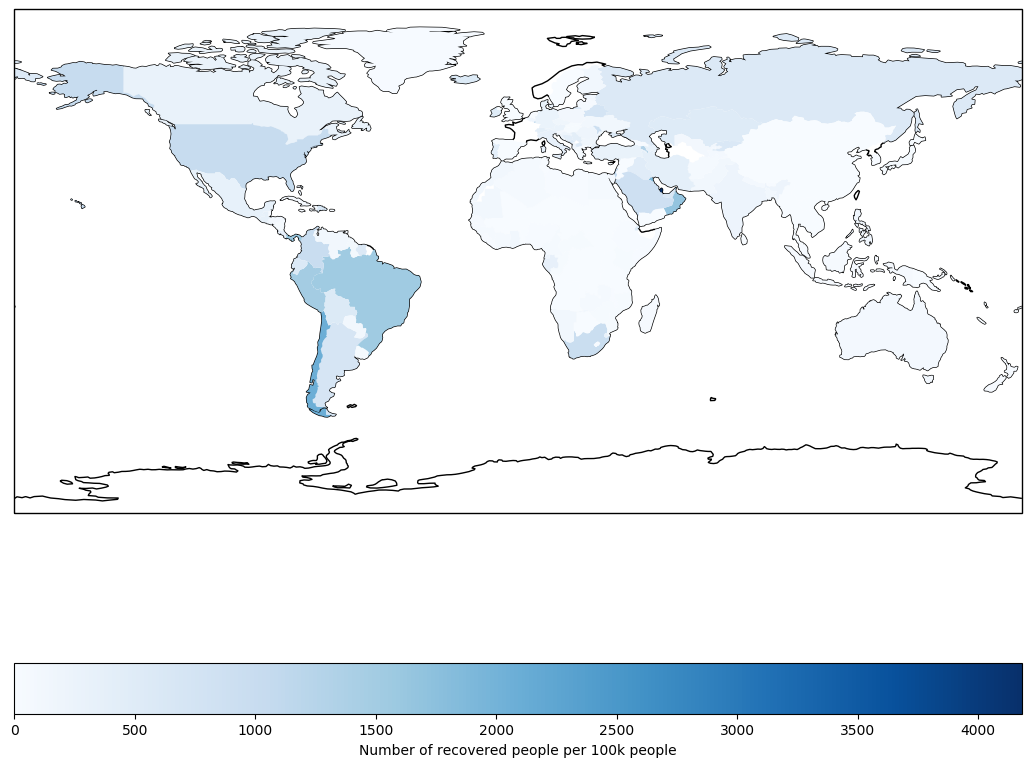
\includegraphics[width=\linewidth]{covid/recovered rate}
	\end{subfigure}
	\begin{subfigure}[b]{0.47\linewidth}
		\includegraphics[width=\linewidth]{covid/death rate}
	\end{subfigure}
	\caption{Covid-19 rates for each country.}
\end{figure}


\begin{figure}[h]
	\centering
	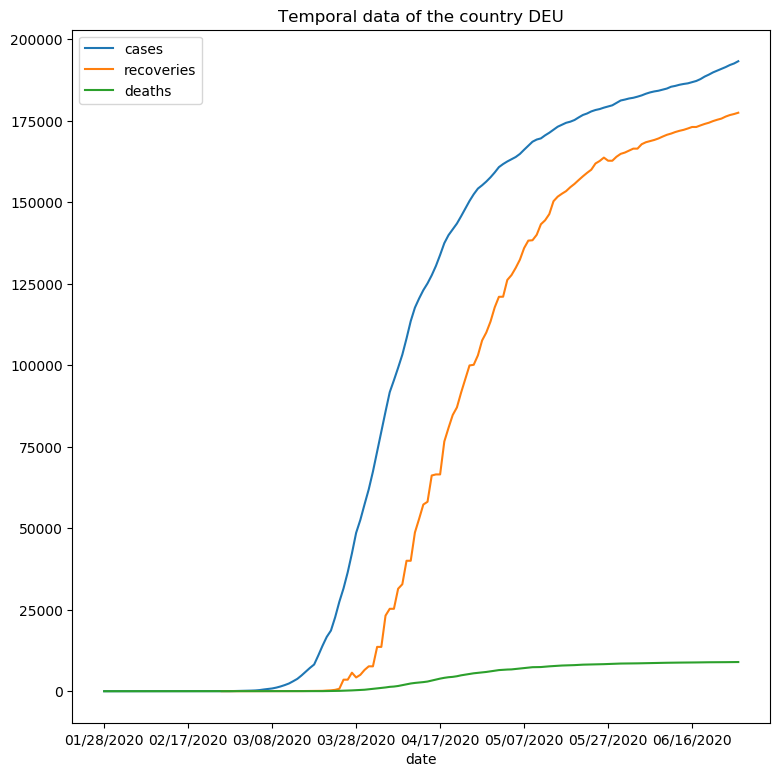
\includegraphics[width=0.50\linewidth]{covid/DEU}
	\caption{Temporal data of Germany. Drawn by using Bing dataset.}
\end{figure}

\subsubsection{Johns Hopkins CSSE}
The second dataset we use is provided by the Center for Systems Science and Engineering (CSSE) at Johns Hopkins University and gathered from multiple sources \cite{JohnsHopkins}.
In our project we access the dataset through https://covid19api.com/, which provides easy access to the dataset, using an API request. Just like the Bing dataset, it includes the number of cases, deaths, recoveries, alongside the coordinates of the
corresponding country or administrative region. This makes it easier to compare them but population data for each country must be taken from another source to calculate the ratio of the statistics to the general population.
According to covid19.com, the dataset is updated multiple times a day. This can be an advantage compared to the dataset of Bing, which is updated daily.


\begin{figure}[h]
	\centering
	\begin{subfigure}[b]{0.47\linewidth}
		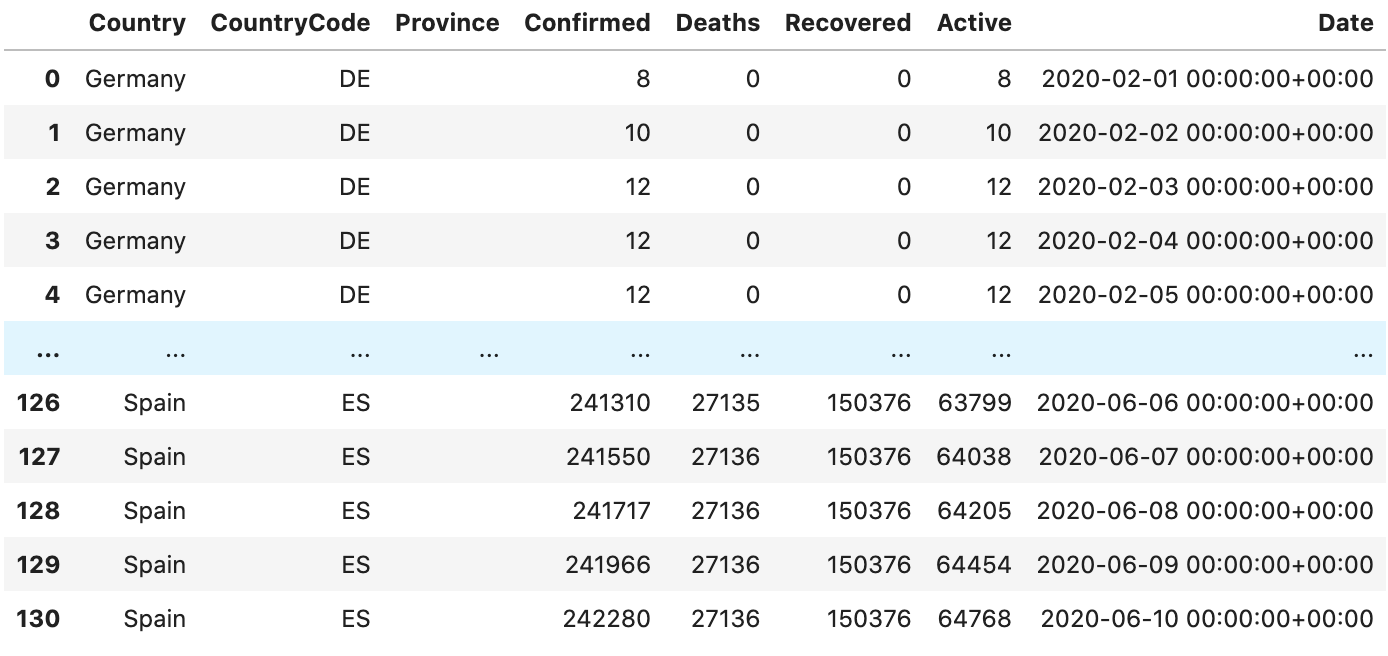
\includegraphics[width=\linewidth]{covid/countrys}
	\end{subfigure}
	\begin{subfigure}[b]{0.47\linewidth}
		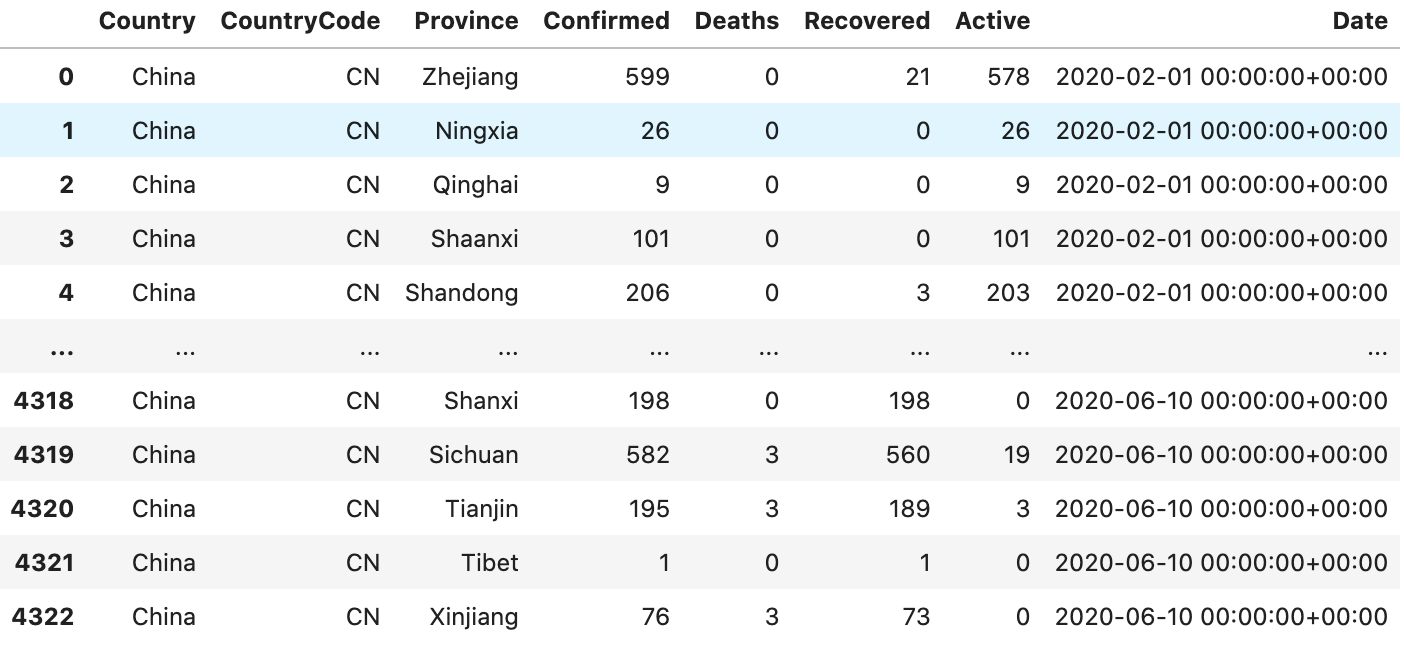
\includegraphics[width=\linewidth]{covid/provinces}
	\end{subfigure}
	\caption{Example of samples from the Johns Hopkins dataset.}
\end{figure}

\subsection{Processing data}

\begin{itemize}
	\item Importing data either online or offline.
	\item Choosing only country-level administrative regions.
	\item Selecting either most recent sample of each country or multiple samples over time for a single country.
	\item Visualizing either recent statistics of all countries or temporal data for a single country.
\end{itemize}
The world maps are drawn with Cartopy \cite{Cartopy}. Other figures are drawn with Matplotlib \cite{Hunter:2007}.

\begin{figure}[h]
	\centering
	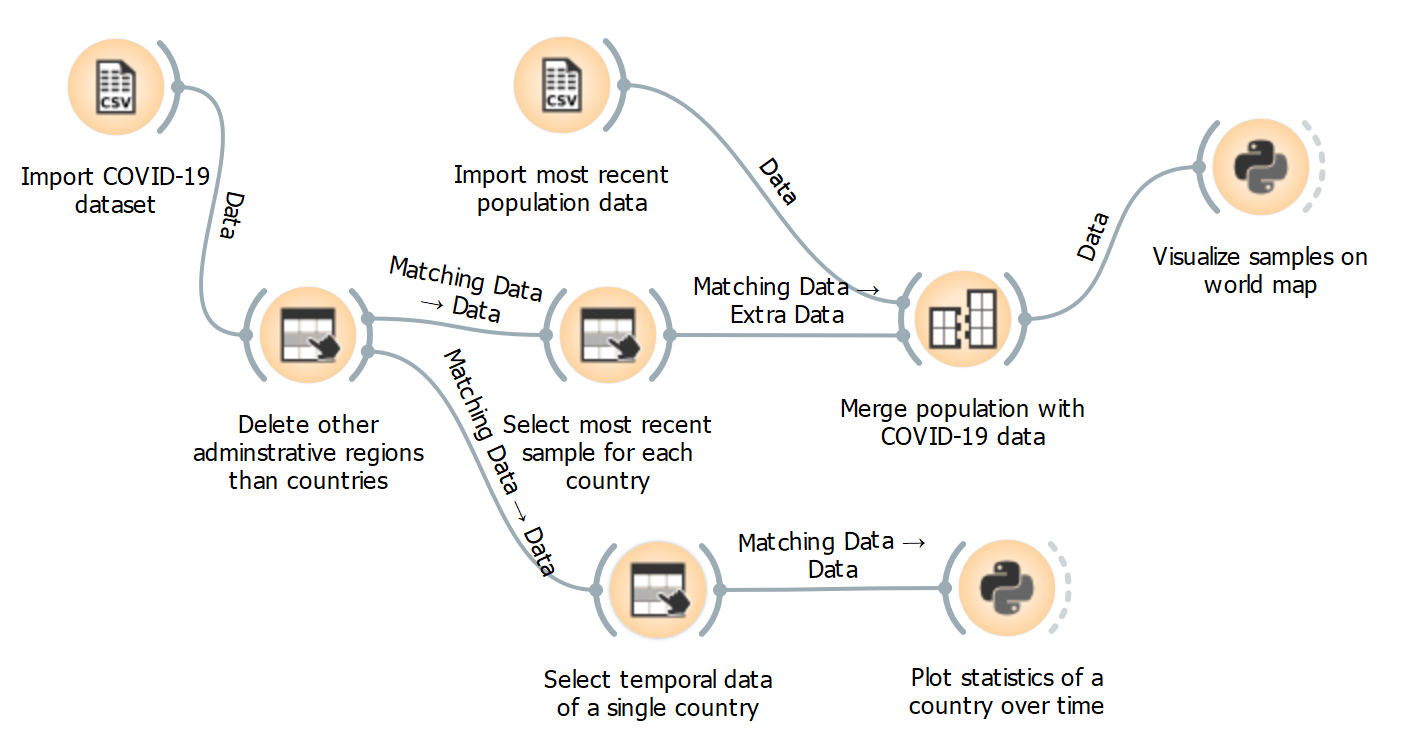
\includegraphics[width=0.80\linewidth]{covid/data_pipeline}
	\caption{Our general pipeline of processing Covid-19 datasets. Drawn using Orange \cite{Orange}}
\end{figure}


\subsection{Conclusion}
Having detailed Covid-19 data is a necessity for our research, since the effect of the pandemic on greenhouse gas emissions will be researched. In the end the datasets we have implemented are frequently updated, easy to access and use, consistent with each other, and have detailed information on cases. Therefore, we don't prefer one dataset over the other. Since we can access temporal data from individual countried throughout the pandemic, it will be easier to model the correlation between Covid-19 cases and greenhouse gas emissions.
\include{../../greenhouse/greenhouse}
\section{Mobility Datasets}

% Why do we need this dataset?
In order to get insights about the possible impact of changed mobility behavior on greenhouse gas emissions, it is important to use different kind of mobility data. The goal by using those datasets is to find a correlation, if there is one, between the mobility behavior and the greenhouse gas emissions. Of course, other aspects that affect the atmospheric greenhouse gas levels also have to be taken into consideration.

% What different sources did you look into and what are their pro's and con's. Are there alternatives?
Mobility behavior relates to various aspects in our life. That's why it is important to have many different kinds of datasets for this topic. Apple and Google recently published mobility reports for almost all countries in the world. Both datasets might be useful in our case due to the fact that they are differently organized. Besides the mobility reports, aviation data might also be interesting to analyze. Since aviation is quite representative for the long-distance travel behavior of the people, this might give some important insights into long-distance traveling compared to regional mobility aspects provided by the mobility reports. To ensure the correctness of the collected aviation data, two different datasets will be used and compared to each other. In the following, the different datasets and the information they contain is explained in a more detailed way.

\begin{itemize}
\item \textbf{Apple Mobility Trends:} \\
The database of Apple's mobility trend report is updated daily and reflects the amount of requests for directions per day in Apple's cards app.\cite{Apple} The data is normalized with a baseline on January 13th, 2020, and shows the further development in percent in respect to this baseline. In total the datasets is split up into data for driving, walking and transit data. This could be extremely useful in our case, since the different kinds of mobility data probably have a different impact on greenhouse gas emissions.

\item \textbf{Google Mobility Report:} \\
The Google mobility reports are structured in a different way. Here, information are given for movement patterns at different categories of geographic places.\cite{Google} The dataset contains information about movement behavior in transit stations, workplaces, parks or retail and recreation. Together with the relationships between different movement patterns and their impact on the atmospheric greenhouse gas level, we will try to find insightful correlations. Determining such correlations, we could predict the impact of an increasing movement behavior after the COVID-19 crises and its impact on the greenhouse gas emissions.

\item \textbf{OpenSky Network Flightlists:}\\
The OpenSky Network provides air traffic data for research topics. The specific dataset we use was updated every month from January 2020 up to May 2020 and hopefully also continues to be updated in the future. It includes data for all flights within this period, including the flight numbers, origin and destination airports and timestamps. The advantage of this dataset is that it contains very detailed data. For example, we could determine the number of flights per day which took off or landed at a specific location. Also, we could determine the number of total flights per day. In this case, we decided to analyze the overall flight hours per day because this is most directly correlated with the greenhouse gas emissions. The disadvantage by using this dataset is that it contains lots of data. Therefore, the pre-processing steps take a relatively large amount of computational resources. The data sources can be found by following this reference: \cite{Opensky}.

\item \textbf{Flightradar24 Tracking Statistics:}\\
Flightradar24 provides historic and live air tracking data. The database is separated into statistics for all flights and only for commercial flights. In each of the cases, the number of flights per day is given as well as a seven-day moving average. This dataset provides helpful insights into the air traffic by day since January 27th, 2020 in a very clear way. The disadvantage of this source is that it does not provide any detailed information about the length of the flights. For example, drone flights are tracked by Flightradar24 which do not affect greenhouse gas emissions. That's why this dataset can only be used in a limited way for our problem, but still it provides some good information about movement patterns in general during the COVID-19 crisis and in the future. In addition, it has to be taken into account that aviation in general affects the overall greenhouse gas emissions only in a small way. The dataset can be found here: \cite{Flightradar24}.

\end{itemize}

% What did you do to prepare the dataset: cleaning, aligning, quality checking, balancing, etc.)

% include plots

% describe them

For all the collected datasets different pre-processing steps had to be taken. In order to get an intuition about the collected data, the goal was to also create plots which present the data in a comprehensible way. All of the pre-processing steps are bundled in a loader class.

The pre-processing of the Apple data mainly consists of specifying the information to extract from the dataset. Therefore it has to be chosen from the three different transport types driving, walking and transit. Additionally, the countries to be extracted have to be specified. If data for the requested country is not available, this country will be ignored in further processing steps. By use of this structure, we are then able to dynamically extract the kind of information we need depending on our future research focus. After extracting the relevant information from the csv file and dropping the irrelevant ones, the data is restructured as a pivot table in order to separate the data by countries and index the samples by date. Missing values are filled with the last valid sample. An exemplary plot for transit data in four European countries is shown in Figure \ref{apple_demo}.

\begin{figure}[h]
\centering
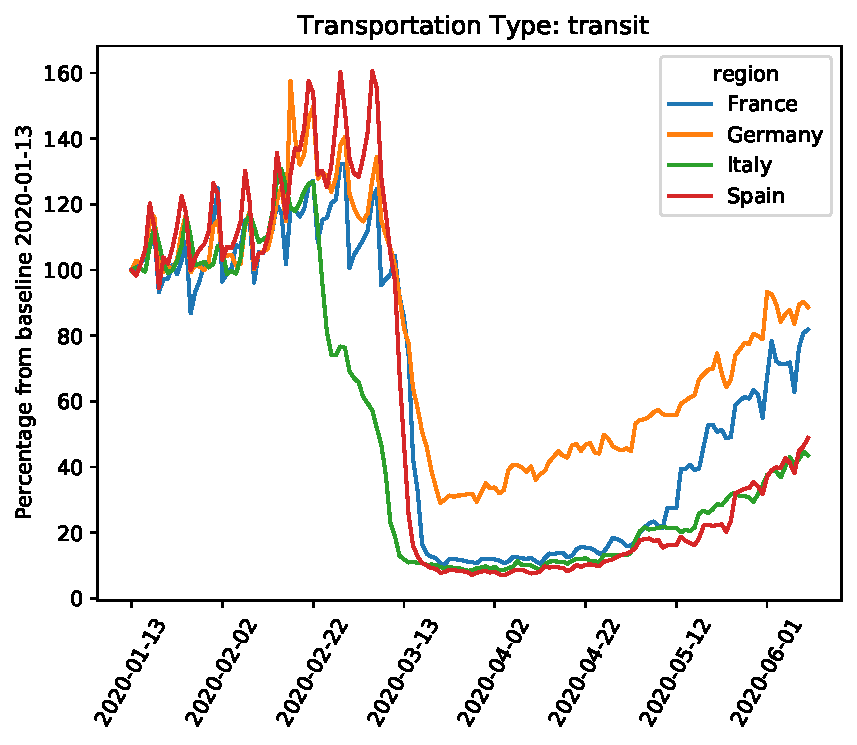
\includegraphics[width=0.5\textwidth]{mobility/apple_demo.pdf}
\caption{Exemplary plot for Apple mobility trend data.}
\label{apple_demo}
\end{figure}

The pre-processing of the Google mobility reports basically follows the same steps. Also the method for handling missing values is the same. In contrast to the Apple datasets, other information types have to be specified here as discussed in the listing above. A demo plot for the movement patterns at workplaces in different European countries is shown in Figure \ref{google_demo}.

\begin{figure}[h]
\centering
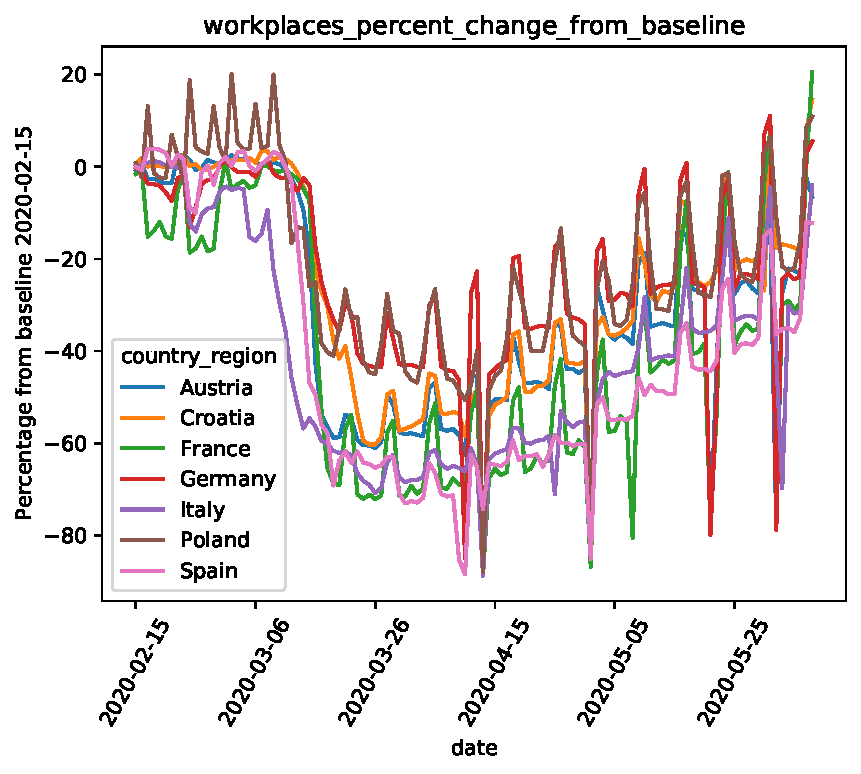
\includegraphics[width=0.5\textwidth]{mobility/google_demo.pdf}
\caption{Exemplary plot for Google mobility report data.}
\label{google_demo}
\end{figure}

Regarding the OpenSky dataset, the pre-processing was computationally more expensive. Since the data were provided in monthly packages, they had to be merged at first. In order to save computational resources, only necessary parts of the dataset were extracted. Since we wanted to extract the overall flight ours per day, the first seen and last seen timestamp was used to calculate the duration of every flight listed in the dataset. Afterwards, a pivot table is created which sums up the flight hours for each day and uses the days as indices. Finally, the day timestamp is modified to only show relevant data. \\
Since these steps take a while when running them on a desktop computer, 
the results were stored in a new csv file containing the overall flight hours per day since January 1st, 2020. The result can be seen in Figure \ref{opensky_demo}.

\begin{figure}[h]
\centering
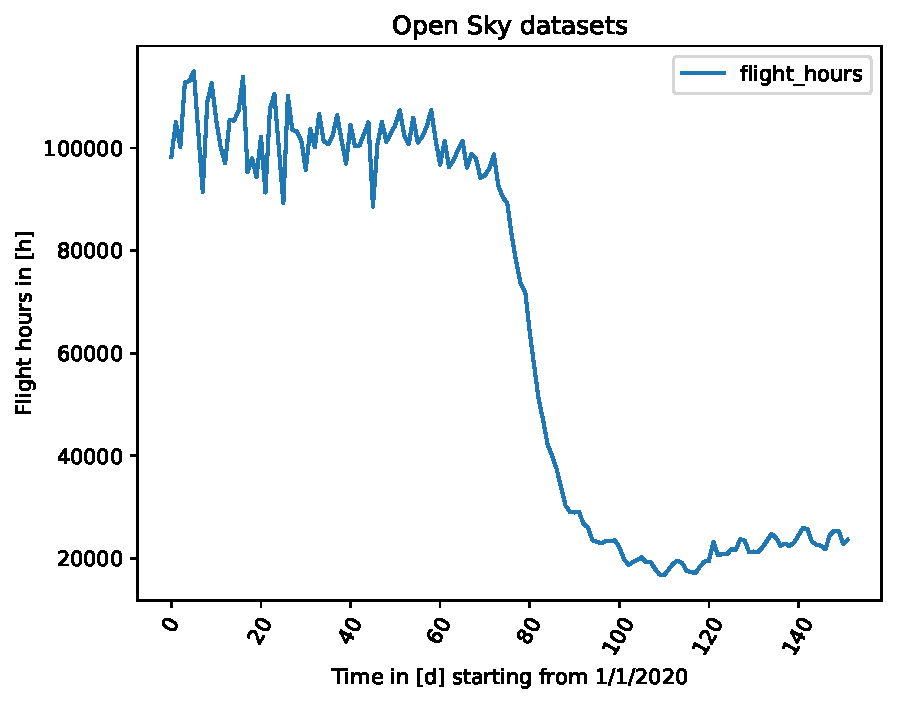
\includegraphics[width=0.5\textwidth]{mobility/opensky_demo.pdf}
\caption{Flight hours per day extracted from the OpenSky datasets.}
\label{opensky_demo}
\end{figure}

The Flightradar24 dataset was already well-prepared. It simply had to be merged into one data frame. The content of this dataset is summarized in Figure \ref{flightradar_demo}. 

\begin{figure}[h]
\centering
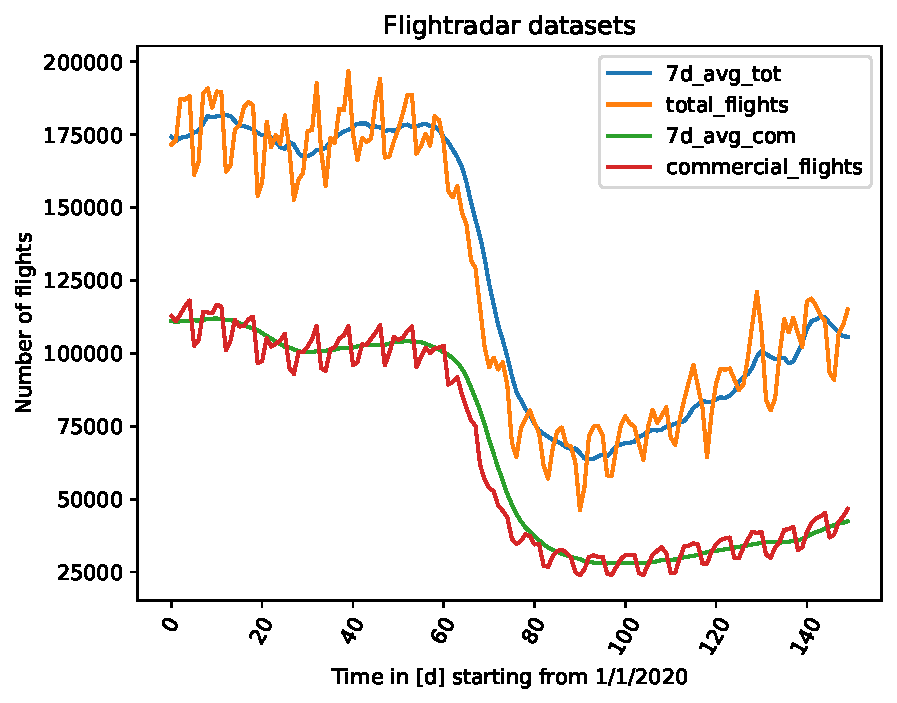
\includegraphics[width=0.5\textwidth]{mobility/flightradar_demo.pdf}
\caption{Number of commercial and total flights provided by Fightradar24.}
\label{flightradar_demo}
\end{figure}

% Check if collected data is useful
All of the collected data might be useful for predicting the influence of COVID-19 on global greenhouse gas emission goals. Especially for predicting the impact in different countries, the mobility report data sets by Apple and Google could be very helpful since they differentiate between movement patterns in different countries. When it comes to transportation, in particular the Apple data set could be very useful because it is separated into different kinds of traveling. This could be extremely useful as different kinds of mobility also have different impacts on greenhouse gas emissions. Together with some side information like the emissions of vehicles, we could try to find correlations between the greenhouse gas levels.

The air traffic data by Flightradar24 has to be reviewed critically. That's because the number of flights does not contain any information about the duration of the flights. Still, it provides an overall intuition about the air traffic and in particular supports the information provided by OpenSky. These datasets could be even more useful since it directly presents how long air planes were flying. Together with the information about average fuel consumption and air plane emissions we can probably use this data to predict the impact of COVID-19 on international climate goals. On the other hand, it has to be taken into consideration that direct emissions from aviation only contribute to about two percent of global emissions \cite{EC_emissions}.

Depending on the machine learning models we are going to use, there will still be some more pre-processing steps required to finally use the datasets for training. One possible strategy to combine the obtained datasets could be to directly take into account the impact of the various contributors to greenhouse gas emissions in percent. This way the information could be combined to one data set. Since we obtained data for various greenhouse gases, this step could also be done for specific greenhouse gases independently in order to improve the accuracy of our predictions. All of the described datasets provide information for roughly the same time interval. The smallest amount of time is covered by the Google data set. That's why an approach for combining the datasets could be to start in February 2020. As it can be seen by inspecting the other datasets which provide information since January 2020, until February the changes in mobility were almost negligible. That's why it will be enough to consider data since February 2020.

% Provide an assessment if you expect the data to be relevant for your project. In what way?
% -> already answered above

\section{International Agreements Datasets}

To investigate to what extent the COVID-19 pandemic will help countries to reach the goals of the international agreements such as the \textit{Paris Agreement under the United Nations Framework Convention on Climate Change}, we needed to find and understand the goals of such agreements. Specifically, we took a closer look at the Paris Agreement and the agreements of the EU. When we researched the agreements of the EU members, we found out that these agreements are incorporated in the Paris agreement. Thus, we focused on gathering data about the Paris Agreement and handle two international agreements at a time.

\subsection{How Does the Paris Agreement Work?}

Basically, the \textit{Paris Agreement} states that every country  ratifying the treaty acknowledges anthropogenic climate change, commits to the well below \SI{2}{\degreeCelsius} and further aims to limit global warming to \SI{1.5}{\degreeCelsius}. To reach these goals, every country has to define its contribution to fight climate change by itself. These so-called \textbf{n}ationally \textbf{d}etermined \textbf{c}ontributions (NDCs) have to be submitted every five years with new, even stricter goals. Furthermore, countries are also allowed to define the same goals in a group, as for example the member of the EU did.

\subsection{Gathering and Pre-processing Data}

The great challenge in finding data about each country's goals, is that every country defines their own goals, without a greater frame. Thus, countries can for example define a cut in greenhouse gas emissions given as a percentage referring to the emissions in a certain year. It is also possible to state a total amount of greenhouse gases a country wants to reduce its emissions. Also, in some NDCs, countries state that they will build more climate-friendly energy plants. Other, mainly less industrialized countries had a mix of unconditioned and conditioned goals. From these few examples, we can already deduce that the data we can gather from the NDCs is highly non-uniform.

Additionally, there is no readily available data about the NDCs. This means, our team would have to read through every NDC and extract the relevant information by hand, consuming an incredible amount of manpower. Luckily, we found a website\footnote{See \url{https://www.carbonbrief.org/paris-2015-tracking-country-climate-pledges}}, in which  all NDCs are summarized to the very core of information. From this, we started to extract the  designated reduction in greenhouse gas emissions for several countries. However, we quickly realized that this would still consume too much man power. Therefore, we decided to only take a closer look at the eight largest contributors, covering more than 70\% of the worlds greenhouse gas emissions in 2017.\footnote{See \url{https://www.worldometers.info/co2-emissions/}} These contributors are China, the US, the EU, India, Brazil, Russia, Japan and Canada in descending order.

Most of the contributors we considered stated a range of emission reduction they aim for. To compare the data more easily, we simply took the mean of minimum and maximum percentage of emission reduction in these cases. Apart from that, the data is rather uniform and we thus did not have to  pre-process it any more. To the data we had from the website\footnote{See \url{https://www.carbonbrief.org/paris-2015-tracking-country-climate-pledges}}, we added the share of \ce{CO2}  emissions in 2012 and 2017 and the total \ce{CO2}  emissions in the referenced year.

\subsection{Data and Plots}

\begin{table}[htb]
	\begin{center}
		\begin{tabular}{lrrrr}
			Country & Share of \ce{CO2} Emissions [\%] & Reduction Goal [\%] & Compared to Year & Fulfill by Year \\\midrule
			China & 24.48 & *62.5 & 2005 & 2030\\
			USA & 13.63 & *27 & 2005 & 2025\\
			EU & 10.94 & 40 & 1990 & 2030\\
			India & 7.18 & *34 & 2005 & 2030\\
			Russia & 4.48 & *27.5 & 2005 & 2025\\
			Japan & 3.35 & 26 & 1990 & 2030\\
			Canada & 1.76 & 30 & 2013 & 2030\\
			Brazil & 1.68 & 37 & 2005 & 2030\\
		\end{tabular}
		\caption{Countries are in descending order by their respective share in global \ce{CO2} emissions in 2017. Greenhouse gas emission reduction goals with an asterisk * are mean values of the range of maximum and minimum reduction goal of the respective country. Further, the year every country refers its reduction goal to and the year by that each country wants to reach its goal is given.}
		\label{tab:data_co2goals}
	\end{center}
	
\end{table}

In \autoref{tab:data_co2goals} we summarized the most important part of the data we gathered for the greenhouse gas emission reduction goals. With this data, we created the plots in \autoref{fig:co2goals_line} and \autoref{fig:co2goals_bubble}. In \autoref{fig:co2goals_line} we simply draw a line from the starting point to the goal of each country. The starting point is at the year each country refers to in its goals, the value is thus set to \SI{100}{\percent} for every respective country. The end point is at the year every country wants to achieve its goals at the height \SI{100}{\percent} minus the reduction goal. The height therefore corresponds to the greenhouse gas emission level each country wants to achieve in the respective year, compared to the year it referred to. From the slopes, we can deduce the rate of greenhouse gas emission reduction in \%/year. This can be used as a measure of how ambitious each country is.

To put the ambitions of each country into perspective, we also need to consider its contribution to the global greenhouse gas emissions. We visualized this in \autoref{fig:co2goals_bubble}, a bubble plot  where the size of each bubble represents the country's share of greenhouse gas emissions. The black line represents the lower boundary of emission reductions to reach the \SI{1.5}{\degreeCelsius} goal\footnote{We need to cut emissions by 45\% by 2030, see \url{https://www.scientificamerican.com/article/global-promises-to-reduce-co2-are-falling-short-of-1-5-degree-c-warming-goal/}}. As we see, only China's goals are ambitious enough to actually reach the \SI{1.5}{\degreeCelsius} goal all countries aim for. Still, the US, the EU and Russia ratified goals that are at least close to the \SI{1.5}{\degreeCelsius} goal. Other countries are less ambitious.

%old plots, not as subplots
%\begin{figure}[htb]
%	\begin{center}
%		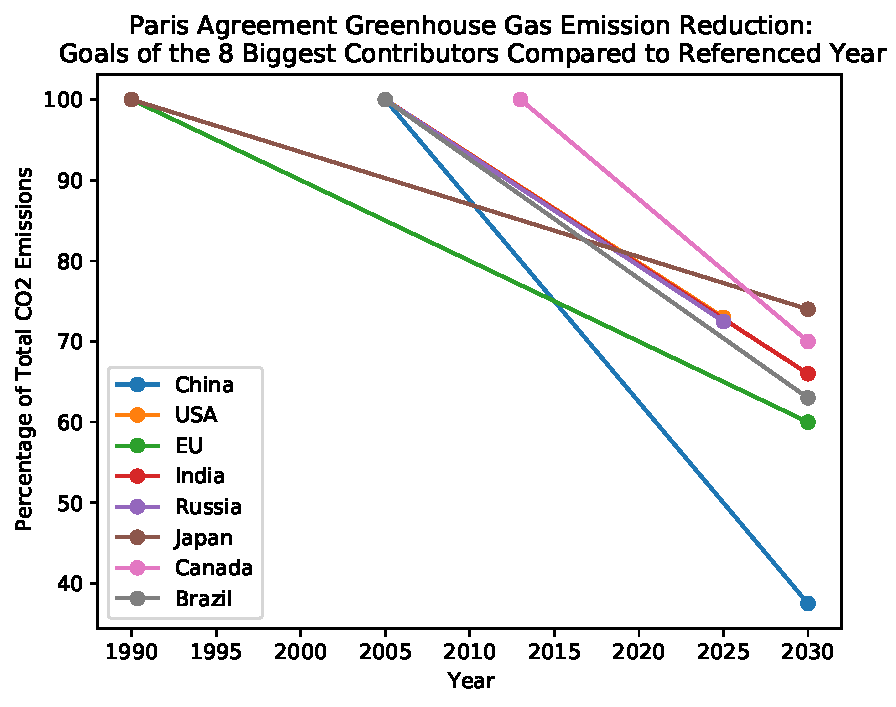
\includegraphics[width=0.8\textwidth]{co2goals/co2goals_lines.pdf}
%		\caption{Line plot for each country's goal compared to the reference year. The $y$-axis represents the greenhouse gas emissions of each country in percent, the $x$-axis the year. Each line starts at (referred  year, 1) and ends at (\(1-\)goal, targeted year). The slopes thus represent the rate of reduction per year in \%/year. This plot does not state anything about absolute data or the contribution of the countries to global greenhouse gas emissions however.}
%		\label{fig:co2goals_line}
%	\end{center}
%\end{figure}
%
%\begin{figure}[htb]
%	\begin{center}
%		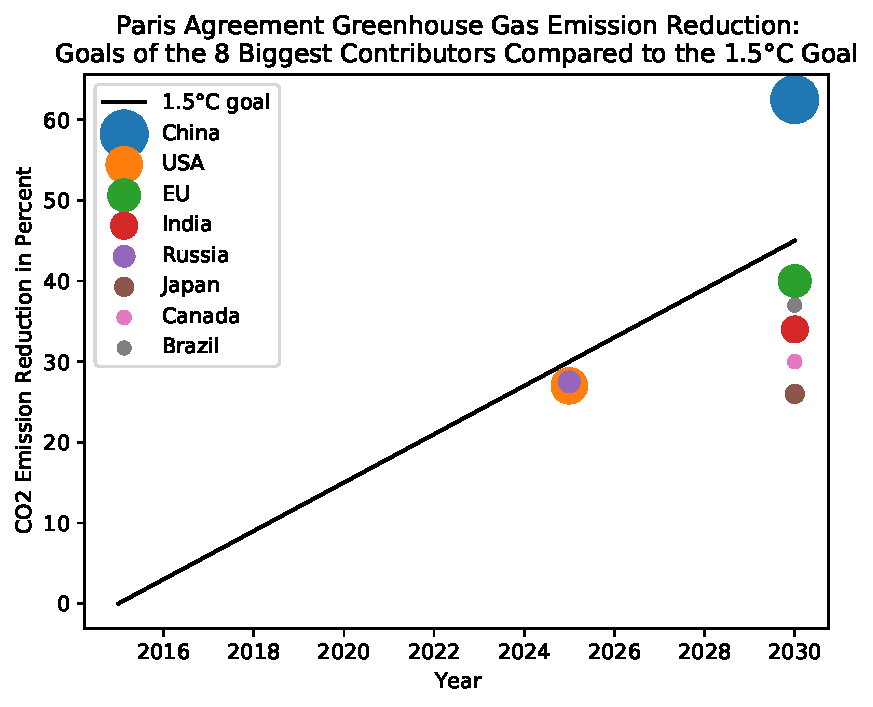
\includegraphics[width=0.8\textwidth]{co2goals/co2goals_bubbles.pdf}
%		\caption{Bubble plot that visualizes how ambitious each country is. The $y$-axis represents the greenhouse gas emission reduction goal in percent, the $x$-axis the year. The size of each bubble corresponds to its share in global greenhouse gas emissions. The black line gives the necessary emission reductions to reach the \SI{1.5}{\degreeCelsius} goal.}
%		\label{fig:co2goals_bubble}
%	\end{center}
%\end{figure}


%\begin{figure}[htb]
%	\begin{center}
%		\begin{subfigure}[b]{0.49\linewidth}
%			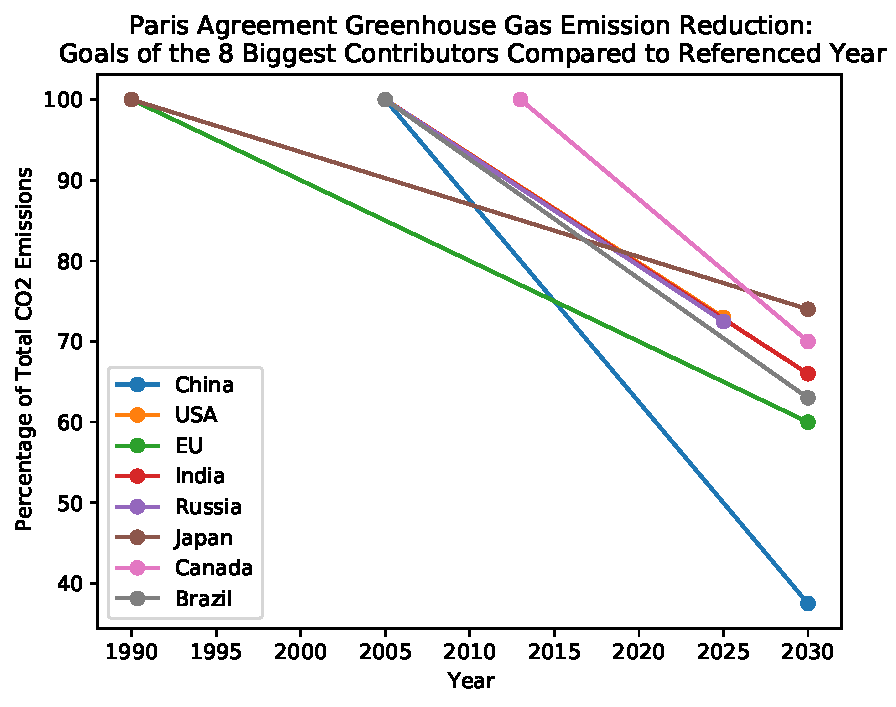
\includegraphics[width=0.8\textwidth]{co2goals/co2goals_lines.pdf}
%			\caption{Line plot for each country's goal compared to the reference year. The $y$-axis represents the greenhouse gas emissions of each country in percent, the $x$-axis the year. Each line starts at (referred  year, 1) and ends at (\(1-\)goal, targeted year). The slopes thus represent the rate of reduction per year in \%/year. This plot does not state anything about absolute data or the contribution of the countries to global greenhouse gas emissions however.}
%			\label{fig:co2goals_line}
%		\end{subfigure}\hfill
%		\begin{subfigure}[b]{0.49\linewidth}
%			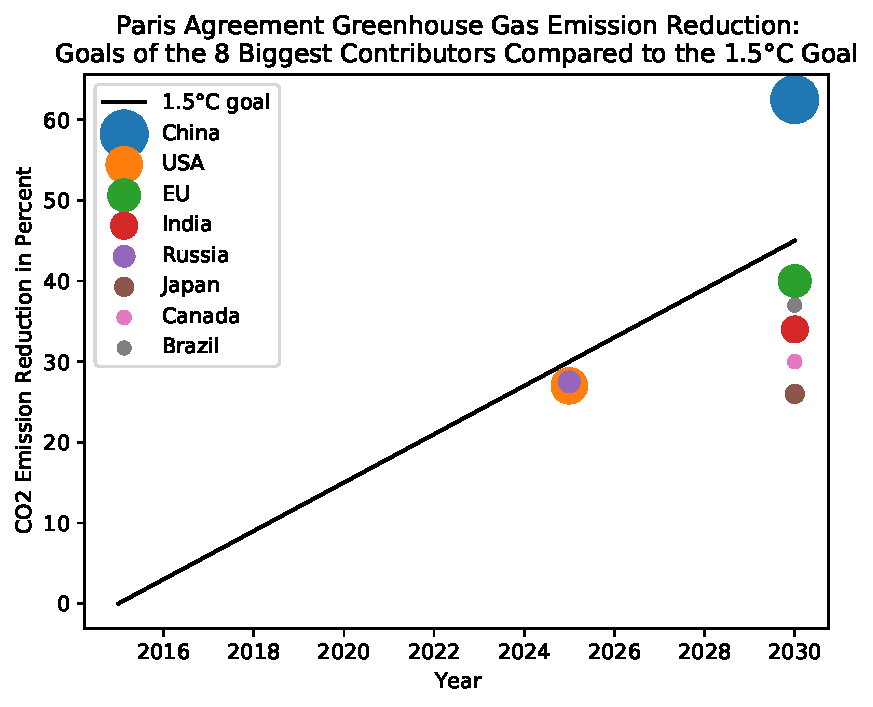
\includegraphics[width=0.8\textwidth]{co2goals/co2goals_bubbles.pdf}
%			\caption{Bubble plot that visualizes how ambitious each country is. The $y$-axis represents the greenhouse gas emission reduction goal in percent, the $x$-axis the year. The size of each bubble corresponds to its share in global greenhouse gas emissions. The black line gives the necessary emission reductions to reach the \SI{1.5}{\degreeCelsius} goal.}
%			\label{fig:co2goals_bubble}
%		\end{subfigure}
%	\end{center}
%\end{figure}









\begin{figure}[htb]
	\begin{center}
		\begin{subfigure}[b]{0.49\linewidth}
			\centering
			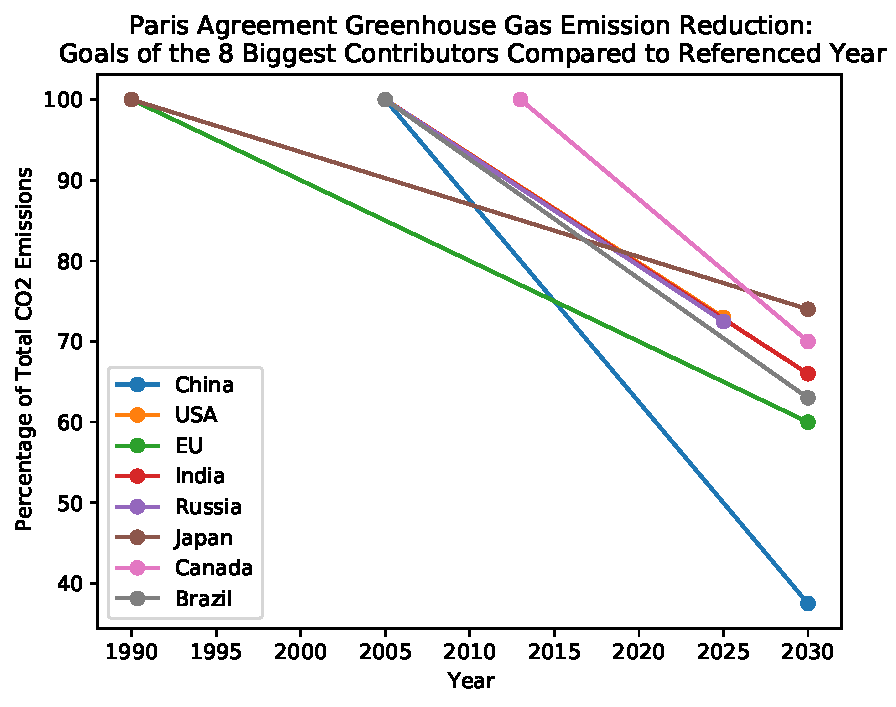
\includegraphics[width=0.8\textwidth]{co2goals/co2goals_lines.pdf}
			\caption{}
			\label{fig:co2goals_line}
		\end{subfigure}\hfill
		\begin{subfigure}[b]{0.49\linewidth}
			\centering
			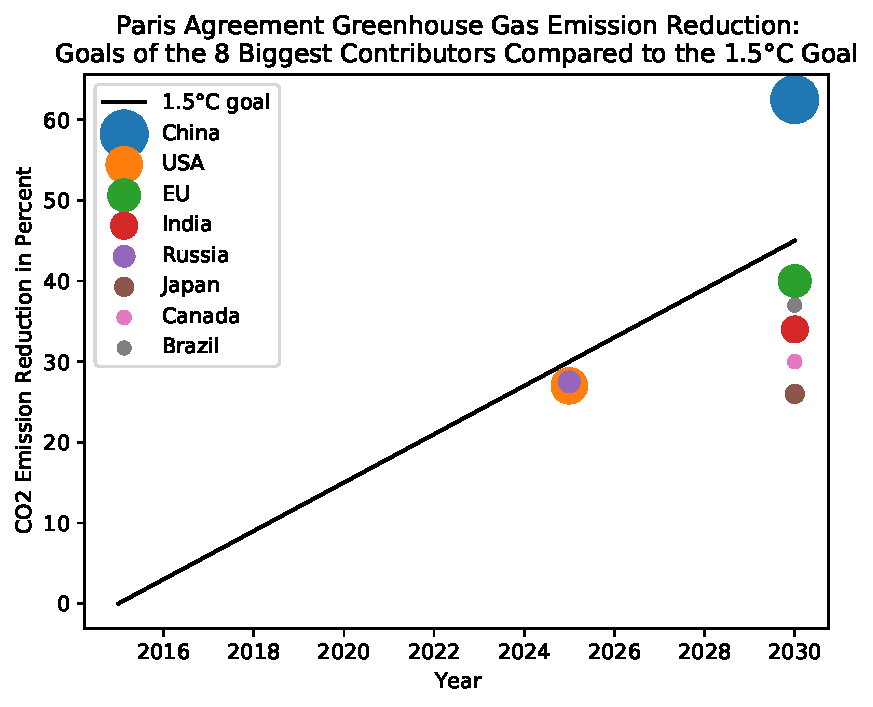
\includegraphics[width=0.8\textwidth]{co2goals/co2goals_bubbles.pdf}
			\caption{}
			\label{fig:co2goals_bubble}
		\end{subfigure}
		\caption{\textbf{a.} Line plot for each country's goal compared to the reference year. The $y$-axis represents the greenhouse gas emissions of each country in percent, the $x$-axis the year. Each line starts at (referred  year, 1) and ends at (\(1-\)goal, targeted year). The slopes thus represent the rate of reduction per year in \%/year. This plot does not state anything about absolute data or the contribution of the countries to global greenhouse gas emissions however.
			\textbf{b.}	Bubble plot that visualizes how ambitious each country is. The $y$-axis represents the greenhouse gas emission reduction goal in percent, the $x$-axis the year. The size of each bubble corresponds to its share in global greenhouse gas emissions. The black line gives the necessary emission reductions to reach the \SI{1.5}{\degreeCelsius} goal.}
	\end{center}
\end{figure}










\subsection{Usage of Emission Reduction Goals Data}
The data we gathered is crucial for our project. With the data, we can compare the greenhouse gas reduction due to the COVID-19 pandemic with the actual goals each country set for itself. From that, we can quantify how much this reduction contributes to the goals. As we have data of the emitters accounting for over two thirds of global greenhouse gas emissions, we not only see how COVID-19 related emission reductions help some individual countries to reach their goals but also see its global impact. For this reason, the data about emission reduction goals -- along with COVID-19 and greenhouse gas emission data -- counts to the most important data sets of our project.






%for \SI{1.5}{\degreeCelsius}, we need to cut emissions by 45\% by 2030\footnote{see \url{https://www.scientificamerican.com/article/global-promises-to-reduce-co2-are-falling-short-of-1-5-degree-c-warming-goal/}}.


% What different sources did you look into and what are their pro's and con's. Are there alternatives?, check

% What did you do to prepare the dataset: cleaning, aligning, quality checking, balancing, etc.), check

% include plots, check

% describe them, check

% Check if collected data is useful, check

% Provide an assessment if you expect the data to be relevant for your project. In what way?, check

%\section{Weather Datasets}

\subsection{Influence of Rain on \ce{CO2}}

Weather plays an important role in air pollution chemistry. Rainy days can make better air quality because of the atmospheric dynamic, which contribute to lower greenhouse gas concentrations in the air, mostly \ce{CO2}. It is known that during global warming the Earth generates more temperature, which means that more water evaporates to the air, and we can expect more rainy days during the year. From one year to another there is hotter and even though the society tries to decrease the \ce{CO2} emission, we have to wait more than 20 years to see the results in our atmosphere. 

We decided to analyse rainfall data in the world during first months in 2020 and try to compare it with trends from the past. This could help us notice how decreasing the \ce{CO2} emission during pandemic can impact on the rainfall in different countries, and also see if there is any impact too. 

\subsection{Finding Rain Data}

The problem was, that data is provided for cities, regions or coordinates, not for all countries. That is why 
firstly, we analyse monthly data from different stations in each country between 1960-1970 years to combine average annual rainfall data for China, USA, Japan, Brazil, Canada, Russia, India and EU. Next step is to find relations between data from first quarter from the past and in 2020. 
This strategy can easily help us to see the main trend, but we still need more specific data, for example, daily measures to see the trends and to try compare it  very accurate. 


\begin{table}[htb]
	\begin{center}
		\begin{tabular}{lrrrr}
			Country & Av. annual rainfall 1960-1990 [mm/day] & Av. 1st. quarter rainfall 1960-1990 [mm/day] & Av. 1st. quarter rainfall 2020 [mm/day] \\\midrule
			China & 747.83 & 181.98 & 162.3 \\
			USA & 918.37 & 264.77 & 206.45 \\
			EU & 708.05 & 162.29 & 158.13 \\
			India & 1512.03 & 188.53 & 105.23\\
			Russia & 479.47 & 88.71 & 94.27 \\
			Japan & 1545.5 & 342.6 & 328.96 \\
			Canada & 858.6 & 178.38 & 165.32 \\
			Brazil & 1446.85 & 566.1 & 634.71 \\
		\end{tabular}
		\caption{Countries are in descending order by their respective share in global \ce{CO2} emissions in 2017. The data shows average annual rainfall between 1960-1990 and average rainfall in first quarter of the same period and 2020.}
		\label{tab:data_weather}
	\end{center}
	
\end{table}

There was no universal source for all countries and it can mean that data may be unreliable. In India for example, the data is very different due to geographic reasons. When data is provided only for cities, this is also pretty difficult and time consuming to prepare good dataset and notice the trends for all countries. rain data is difficult to handle quantitatively, so looking for trends and handle data qualitatively makes more sense

\subsection{Data for Rain Fall Data}

The best dataset which provide reliable, easy accessible data is rainfall for coordinates. In our one set there is data where we can find coordinates, date and rainfall. 

\begin{figure}[htb]
	\begin{center}
		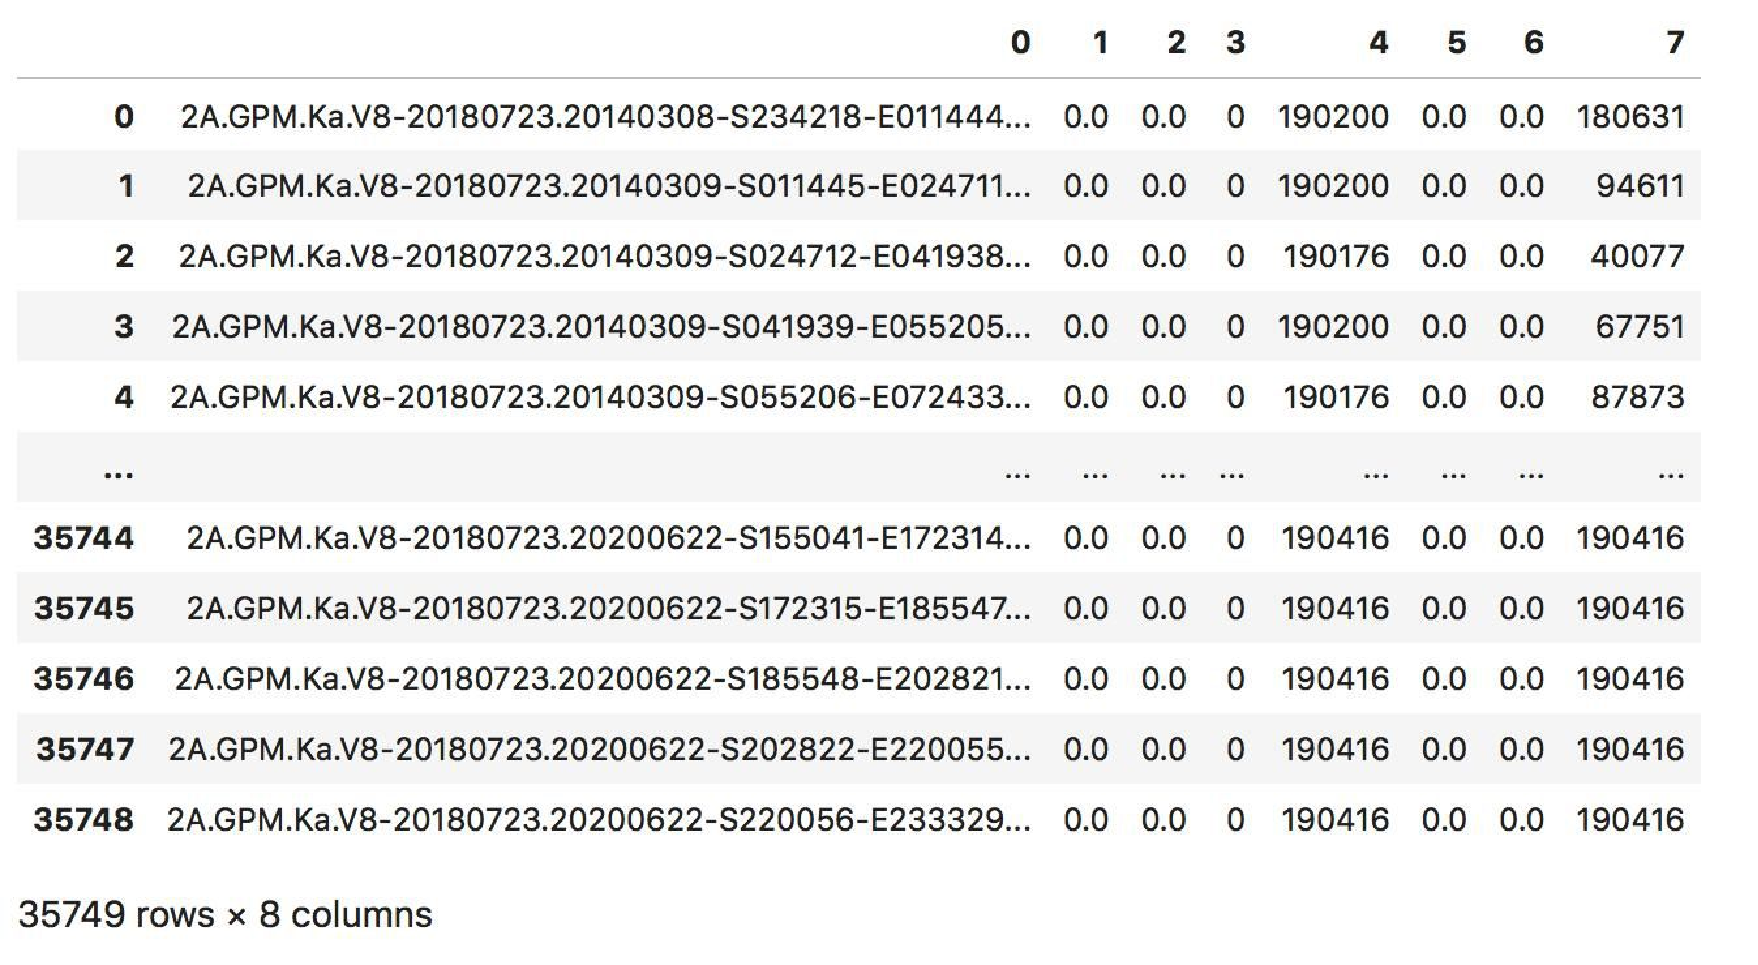
\includegraphics[width=0.8\textwidth]{weather/weather_data.pdf}
		\caption{weather data for separate coordinates.}
		\label{fig:Here we can find lot's of data and some of them are irrelevant to us. In column one we notice coordinates and date.}
	\end{center}
\end{figure}

We prepared algorithm to separate informations only for relevant ones from the first column. Now we have two coordinates separately and also the date for a measurement. 

\begin{figure}[htb]
	\begin{center}
		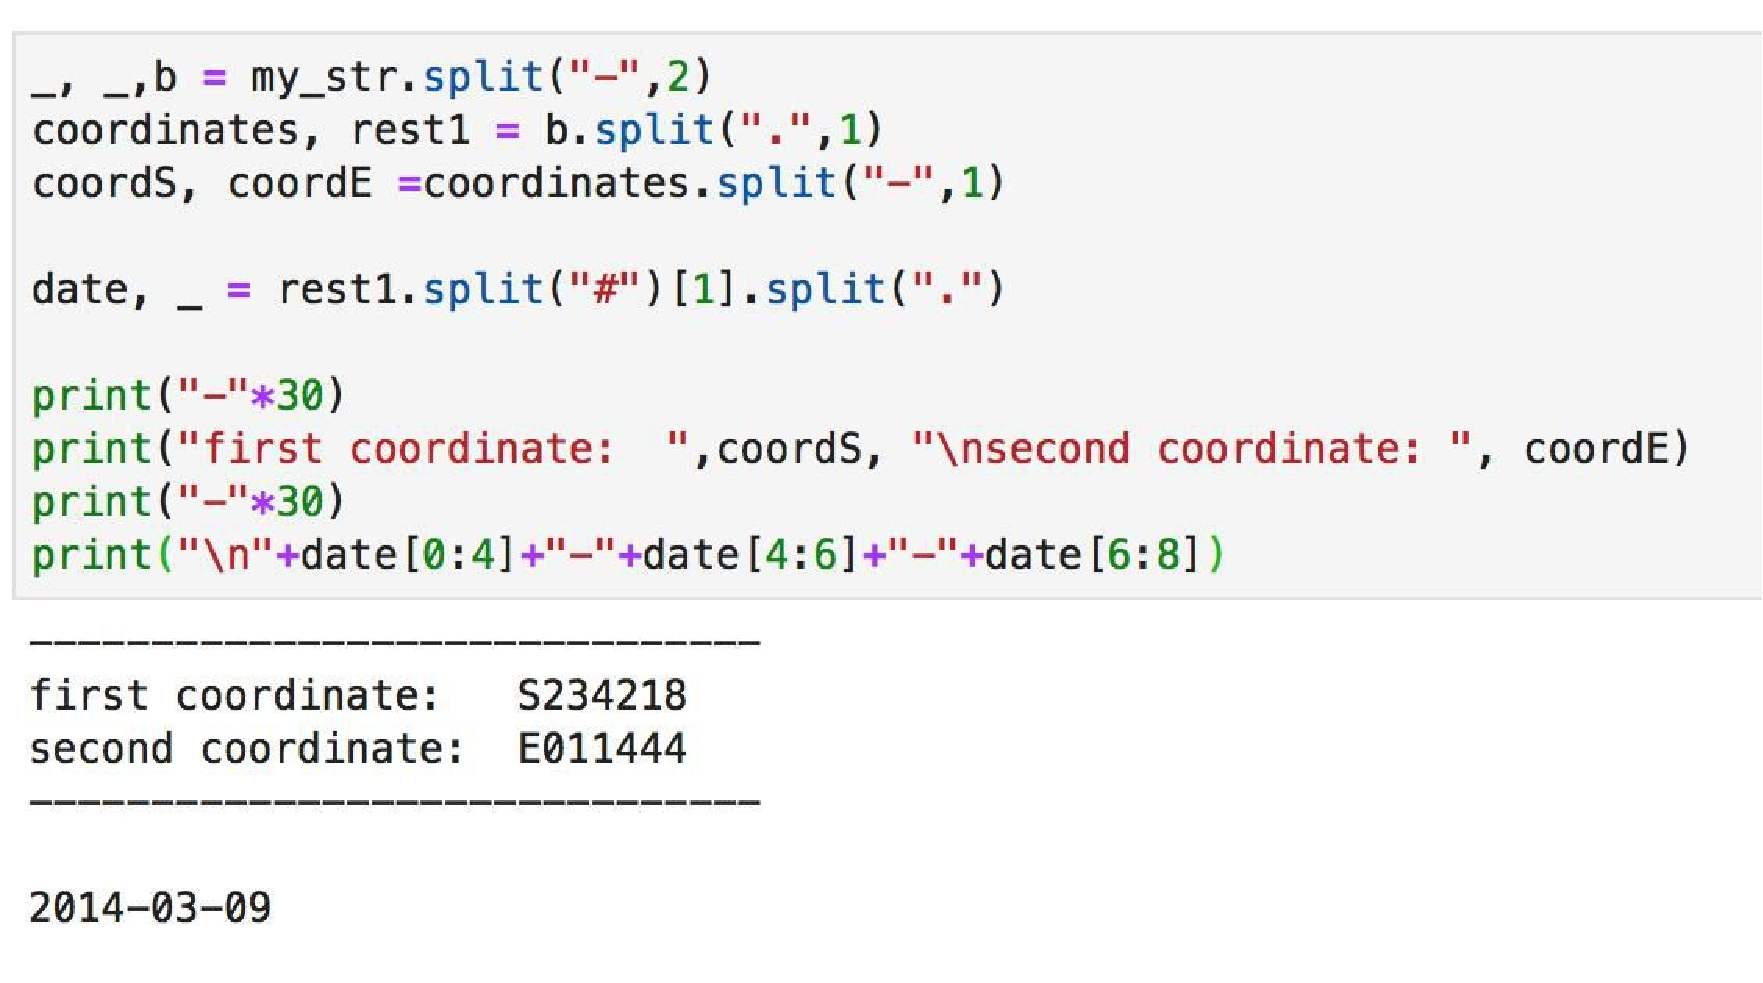
\includegraphics[width=0.8\textwidth]{weather/weather_split_data.pdf}
		\caption{Here we provide algorithm to access only relevant data from the first column such as coordinates and date. .}
		\label{fig:pSeparate coordinates and date}
	\end{center}
\end{figure}

Next step is to combine these coordinates, dates and rainfall data to show the trends. We also have knowledge how to find countries using coordinates in Python, which is very useful. The problem is that we don't know the unit of these coordinates. There are three common units - decimal degrees (DD), degrees-decimal-minutes (DDM) and degrees-minutes-seconds (DMS), but our coordinates are in different units. Also there are only coordinates for one quarter of the world (SE) and we need to find an idea how to calculate it and make it accessible to our algorithm. Since we don't know how to calculate these coordinates, we can't use it. 




\section{Conclusion and Outlook}

In summary, we have gathered data concerning four big aspects that are important for answering to what extent the Covid-19 pandemic will contribute towards reaching the  goals stated in the Paris Agreements. Each dataset was found to be crucial for solving the task. To conclude this overview, we list our main decisions and findings:

%covid
\textbf{COVID-19:}
\begin{itemize}
	\item Frequently updated datasets with high temporal resolution per country.
	\item Preferred datasets: \textbf{Bing}, \textbf{Johns Hopkins CSSE}.
\end{itemize}


%greenhouse gases
\textbf{Greenhouse Gases:}
\begin{itemize}
	\item The datasets discriminate by type of gas, spatially, temporal and by industry sector with reasonable resolution.
	\item Preferred datasets: \textbf{Global Monitoring Laboratory}, \textbf{Emissions Database for Global Atmospheric Research}.
\end{itemize}

%mobility
\textbf{Mobility:}
\begin{itemize}
	\item By using the datasets, correlations of regional and global transport with greenhouse gas measurements are accessible.
	\item Preferred datasets: \textbf{Apple Mobility}, \textbf{Google Mobility}, \textbf{OpenSky}.
\end{itemize}

%international agreements
\textbf{International Agreements:}
\begin{itemize}
	\item The biggest eight contributors (including EU) covered more than 70\% of the worlds greenhouse gas emissions in 2017, and are therefore most relevant for the project. 
	\item The scope was limited to their specific goals, as we had to create our own dataset from unformatted information.
\end{itemize}

%Outlook
To address our research question even better, we have already attempted to access weather data from NASA satellites, as we want to quantify the influence of precipitation on emission measurements. All datasets mentioned above are already accessible as a pandas dataframe in our repository. With these datasets, we feel confident to start implementing a model.






\bibliographystyle{unsrt}
\bibliography{references,references_mobility,references_greenhouse,references_covid}  %%% Remove comment to use the external .bib file (using bibtex).
%%% and comment out the ``thebibliography'' section.


%%% Comment out this section when you \bibliography{references} is enabled.



\end{document}
